\documentclass{article}

\usepackage[a4paper,margin=2.5cm]{geometry}
\usepackage{amsmath}
\usepackage{amssymb}
\usepackage{fancyhdr}
\usepackage{tikz}
\usepackage{float}
\usepackage{MnSymbol,wasysym}
\usetikzlibrary{arrows}

\newcommand{\tE}[1]{$\mathbb{E}[\mbox{#1}]$}
\newcommand{\E}[1]{\mathbb{E}[\mbox{#1}]}

\pgfsetxvec{\pgfpoint{12cm}{0cm}}

\title{\vspace{-2cm}ECON20005 Assignment 3}
\date{\today}
\author{Lucas Fern (1080613)\\Friday 12:00pm Tutorial}

\lhead{ECON20005 - Assignment 3}
\rhead{Lucas Fern (1080613)}
\pagestyle{fancy}

\begin{document}
\maketitle
\section*{Question 1: Entry Deterrence}
\subsection*{1.1}
When the firms set quantities simultaneously it is an example of Cournot competition. Since firms $A$ and $B$ are the only ones in the market, $Q = q_{A} + q_{B} \implies P = 25 - (q_{A} + q_{B})$.\\[2mm]
Firm A has profit $\Pi_{A} = P \times q_{A} - c_{A} \times q_{A} = (25 - q_{A} - q_{B}) q_{A} - 5 \times q_{A} = 20q_{A} - q_{A}^{2} - q_{A}q_{B}$.\\[2mm]
Maximising with respect to $q_{A}$:
\begin{align*}
    \frac{\partial \Pi_{A}}{\partial q_{A}} &= 20 - 2q_{A} - q_{B} = 0\\
    q_{A} &= \frac{20 - q_{B}}{2}
\end{align*}
Since the firms are subject to identical conditions:
$$q_{B} = \frac{20 - q_{A}}{2}$$
Substituting $B$'s best response quantity into $A$'s:
\begin{align*}
    q_{A} &= \frac{20 - \frac{20 - q_{A}}{2}}{2}\\
    &= \frac{\frac{20 + q_{A}}{2}}{2}\\
    &= \frac{20 + q_{A}}{4}\\
    0 &= 20 - 3q_{A}\\
    q_{A} &= \frac{20}{3}
\end{align*}
Because the firms face symmetric best response quantities, $q_{A} = q_{B} \implies q_{B} = \frac{20}{3}$.
Substituting this back into the profit function:
\begin{align*}
    \Pi_{A} = 20q_{A} - q_{A}^{2} - q_{A}q_{B} &= 20 \cdot \frac{20}{3} - \left( \frac{20}{3} \right)^{2} - \left( \frac{20}{3} \right)^{2}\\
    &= \frac{400}{9}
\end{align*}
So the equilibrium quantities are $q_{A} = q_{B} = \frac{20}{3}$ and the equilibrium profits are $\Pi_{A} = \Pi_{B} = \frac{400}{9}$.

\subsection*{1.2}
Since $B$ is the second mover, their response will depend on firm $A$, from Q1.1 we have
$$q_{B} = \frac{20 - q_{A}}{2}.$$
Doing backward induction with this, firm $A$'s optimal choice can be found by taking the first order condition of the profit function and setting equal to zero:
\begin{align*}
    \Pi_{A} = 20q_{A} - q_{A}^{2} - q_{A}q_{B} &= 20q_{A} - q_{A}^{2} - q_{A}\frac{20 - q_{A}}{2}\\
    &= 10q_{A} - \frac{q_{A}^{2}}{2}\\
    \frac{\partial \Pi_{A}}{\partial q_{A}} = 10 - q_{A} &= 0\\
    q_{A} &= 10
\end{align*}
Then to find $B$'s quantity:
\begin{align*}
    q_{B} &= \frac{20 - q_{A}}{2}\\
    &= \frac{20 - 10}{2}\\
    q_{B} &= 5
\end{align*}
So the total market quantity is $q_{A} + q_{B} = 15$, making the market price $25 - 15 = 10$. This means $A$'s profit is:
$$\Pi_{A} = P \times q_{A} - c_{A} \times q_{A} = 10 \times 10 - (5 \times 10) = 50$$
and B's profits are:
$$10 \times 5 - (5 \times 5) = 25.$$
The equilibrium quantities and profits differ from Q1.1 because as the first mover $A$ is able to commit to producing a larger quantity knowing that the best way for $B$ to respond is by producing less. $A$ partially pushes $B$ out of the market.

\subsection*{1.3}
Taking $B$'s profit equation and subtracting the fixed entry cost:
$\Pi_{B} = P \times q_{B} - c_{B} \times q_{B} - F = 20q_{B} - q_{B}^{2} - q_{A}q_{B} - 9.$
Importantly, since the derivative of the constant fixed cost is 0, $B$'s best response doesn't change, so substituting in $B$'s best response from Q1.1 in:
\begin{align*}
    \Pi_{B} &= 20q_{B} - q_{B}^{2} - q_{A}q_{B} - 9\\
    &= 20 \times \frac{20 - q_{A}}{2} - \left( \frac{20 - q_{A}}{2} \right)^{2} - q_{A} \times \frac{20 - q_{A}}{2} - 9\\
    &= 200 - 10q_{A} - (100 - 10q_{A} + q_{A}^{2}/4) - 10q_{A} + q_{A}^{2}/2 - 9\\
    &= 91 - 10q_{A} + q_{A}^{2}/4
\end{align*}
Therefore for $B$ to not enter the market, $91 - 10q_{A} + q_{A}^{2}/4$ must be less than or equal to 0.
\begin{align*}
    91 - 10q_{A} + q_{A}^{2}/4 &\leq 0\\
    q_{A}^{2} - 40q_{A} + 364 &\leq 0\\
    (q_{A} - 14)(q_{A} - 26) &\leq 0
\end{align*}
Since the equation for $\Pi_{B}$ is a positive quadratic, $B$'s profit is 0 or negative for $q_{A} \in [14, 26]$, so the minimum quantity $A$ can choose to push $B$ out of the market is $q_{A} = 14$.

\subsection*{1.4}
$A$'s profit when $B$ enters the market in Q1.2 is 50. In Q1.3 where $A$ pushes $B$ out of the market, $A$ sells a quantity $q_{A} = 14$. With $A$ being the only firm in the market, the price is $P = 25 - 14 = 11$, so $A$'s profit is $\Pi_{A} = 11 \times 14 - 5 \times 14 = 84$. $84 > 50$ so it is profit maximising for $A$ to deter $B$ from entering the market.

\section*{Question 2: Twists on the Linear City and Ice-Cream Salesman Models}
\subsection*{2.1}
Let the consumer indifferent between $A$ and $B$ be located at position $x_{1} \in [0, 0.5]$, their travel cost per unit distance is $t=3$ so the indifference condition is:
\begin{align*}
    p_{A} + 3x_{1} &= p_{B} + 3(0.5 - x_{1})\\
    6x_{1} &= p_{B} - p_{A} + 1.5\\
    x_{1} &= \frac{p_{B} - p_{A} + 1.5}{6}
\end{align*}
Then if the consumer indifferent between $B$ and $C$ is located at $x_{2} \in [0.5, 1]$, their indifference condition is:
\begin{align*}
    p_{B} + 3(x_{2} - 0.5) &= p_{C} + 3(1 - x_{2})\\
    6x_{2} &= p_{C} - p_{B} + 4.5\\
    x_{2} &= \frac{p_{C} - p_{B} + 4.5}{6}
\end{align*}
If $x_{1}$ or $x_{2}$ are out of their defined boundaries then no indifferent consumer exists in that section of the city.

\subsection*{2.2}
Starting with firm $A$, their profit is equal to the amount of consumers they sell to times the price, minus their cost:
\begin{align*}
    \Pi_{A} &= 100 \times x_{1} \times (p_{A} - c)\\
    &= 100(p_{A} - 1) \times \frac{p_{B} - p_{A} + 1.5}{6}
\end{align*}
Maximising their profit by setting the first order condition equal to zero:
\begin{align*}
    \frac{\partial \Pi_{A}}{\partial p_{A}} = 100(p_{A} - 1) \times \frac{-1}{6} + 100 \times \frac{p_{B} - p_{A} + 1.5}{6} &= 0\\
    \frac{100 - 100p_{A}}{6} + \frac{100p_{B} - 100p_{A} + 150}{6} &= 0\\
    \frac{250 - 200p_{A} + 100p_{B}}{6} &= 0\\
    250 + 100p_{B} &= 200p_{A}\\
    p_{A} &= \frac{5 + 2p_{B}}{4}
\end{align*}
Now the same for firm $B$ but considering that they get customers from both ends of the street:
\begin{align*}
    \Pi_{B}&= 100 \times (x_{2} - x_{1}) \times (p_{B} - c)                                                      \\
           &= 100(p_{B} - 1) \times \left( \frac{p_{C} - p_{B} + 4.5}{6} - \frac{p_{B} - p_{A} + 1.5}{6} \right) \\
           &= 100(p_{B} - 1) \times \left( \frac{p_{A} - 2p_{B} + p_{C} + 3}{6} \right)                          \\
\end{align*}
\begin{align*}
    \frac{\partial \Pi_{B}}{\partial p_{B}} = 100(p_{B} - 1) \times \frac{-1}{3} + 100 \times \frac{p_{A} - 2p_{B} + p_{C} + 3}{6} & = 0\\
    \frac{200 - 200p_{B}}{6} + \frac{100p_{A} - 200p_{B} + 100p_{C} + 300}{6} & = 0\\
    \frac{500 + 100p_{A} - 400p_{B} + 100p_{C}}{6} & = 0\\
    500 + 100p_{A} + 100p_{C} &= 400p_{B}\\
    p_{B} &= \frac{5 + p_{A} + p_{C}}{4}
\end{align*}
Since the location of consumers and firms on the street is symmetric about the centre, the firms face identical costs, and because typesetting \LaTeX\ takes longer than I'd like to admit, we will use the symmetry to conclude that firm $C$'s best response price is equal to firm $A$'s, therefore
$$p_{C} = \frac{5 + 2p_{B}}{4}.$$
Next, solving for the equilibrium prices, start with $B$:
\begin{align*}
    p_{B} &= \frac{5 + p_{A} + p_{C}}{4}\\
    &= \frac{5 + \frac{5 + 2p_{B}}{4} + \frac{5 + 2p_{B}}{4}}{4}\\
    &= \frac{30 + 4p_{B}}{16}\\
    16p_{B} &= 30 + 4p_{B}\\
    12p_{B} &= 30\\
    p_{B} &= 2.5
\end{align*}
Then
$$p_{A} = p_{C} = \frac{5 + 2p_{B}}{4} = \frac{10}{4} = 2.5.$$
So all firms charge a price equal to 2.5 at equilibrium.\\[2mm]
Finally to find the profits:
\begin{align*}
    100(p_{A} - 1) \times \frac{p_{B} - p_{A} + 1.5}{6} &= 100(2.5 - 1) \times \frac{2.5 - 2.5 + 1.5}{6}\\
    &= 150 \times \frac{1.5}{6}\\
    &= 37.5
\end{align*}
So by symmetry $\Pi_{C}$ also equals 37.5, and:
\begin{align*}
    \Pi_{B} &= 100(p_{B} - 1) \times \left( \frac{p_{A} - 2p_{B} + p_{C} + 3}{6} \right)\\
    &= 150 \times \frac{3}{6}\\
    &= 75
\end{align*}
So although all firms charge identical prices, $B$'s location in the middle of the street allows them to attract twice as many customers as the other firms, giving them twice the profits.

\subsection*{2.3}
Firstly, since $p=20$ is greater than their cost $c=1$, all firms maximise their profit by attracting the most consumers. Since all prices are equal and the cost of travel for a consumer is constant along the whole street, consumers simply purchase from the closest firm.\\[2mm]
With firms located at 0, 0.5, and 1, the indifferent consumers are located at $\frac{0 + 0.5}{2} = 0.25$ and $\frac{0.5 + 1}{2} = 0.75$, meaning that firm $A$ captures the consumers in $[0, 0.25)$, firm $B$ gets $(0.25, 0.75)$ and the consumers in $(0.75, 1]$ purchase from $C$. In this situation if $A$ moves to position 0.1, then the midpoint and therefore indifferent consumer between $A$ and $B$ is located at $\frac{0.1 + 0.5}{2} = 0.3$, so $A$ captures the region $[0, 0.3)$ by unilaterally deviating to position 0.1 (since there is no firm to $A$'s ``left'' that they lose space to by moving). By doing this $A$ increases their market share from 25\% to 30\%, and since sales are profitable $A$ therefore increases their profit by unilaterally deviating, so setting up at 0, 0.5 and 1 cannot be a Nash equilibrium when $p=20$.

\subsection*{2.4}
In the scenario with firms placed at 0, 1/2 and 1, the firms divide the market into these intervals, where the arrows point to a consumer's nearest firm:
\begin{figure}[H]
    \centering
    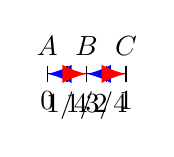
\begin{tikzpicture}
        \draw[] (0,0) -- (1,0) ; %edit here for the axis
        \foreach \x in  {0,1/4,1/2,3/4,1} % edit here for the vertical lines
        \draw[shift={(\x,0)},color=black] (0pt,3pt) -- (0pt,-3pt);
        \foreach \x in {0,1/4,1/2,3/4,1} % edit here for the numbers
        \draw[shift={(\x,0)},color=black] (0pt,0pt) -- (0pt,-3pt) node[below] 
        {$\x$};

        \draw[shift={(0,0)},color=black] (0pt,0pt) -- (0pt, 3pt) node[above] 
        {$A$};
        \draw[shift={(1/2,0)},color=black] (0pt,0pt) -- (0pt, 3pt) node[above] 
        {$B$};
        \draw[shift={(1,0)},color=black] (0pt,0pt) -- (0pt, 3pt) node[above] 
        {$C$};

        \draw[latex-, line width=2pt,blue] (0,0) -- (1/4,0);
        \draw[-latex, line width=2pt,red] (1/4,0) -- (1/2,0);
        \draw[latex-, line width=2pt,blue] (1/2,0) -- (3/4,0);
        \draw[-latex, line width=2pt,red] (3/4,0) -- (1,0);
    \end{tikzpicture}
\end{figure}
\noindent The four intervals are of equal length, so the average travel distance for the entire linear city is the same as the average travel distance for one segment; $\frac{1}{4} \div 2 = \frac{1}{8}$.\\[2mm]
In the other scenario with firms at 1/4, 1/2 and 3/4, the market is divided like this:
\begin{figure}[H]
    \centering
    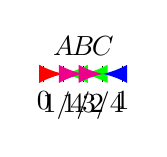
\begin{tikzpicture}
        \draw[] (0,0) -- (1,0) ; %edit here for the axis
        \foreach \x in  {0,1/4,1/2,3/4,1} % edit here for the vertical lines
        \draw[shift={(\x,0)},color=black] (0pt,3pt) -- (0pt,-3pt);
        \foreach \x in {0,1/4,1/2,3/4,1} % edit here for the numbers
        \draw[shift={(\x,0)},color=black] (0pt,0pt) -- (0pt,-3pt) node[below] 
        {$\x$};

        \draw[shift={(1/4,0)},color=black] (0pt,0pt) -- (0pt, 3pt) node[above] 
        {$A$};
        \draw[shift={(1/2,0)},color=black] (0pt,0pt) -- (0pt, 3pt) node[above] 
        {$B$};
        \draw[shift={(3/4,0)},color=black] (0pt,0pt) -- (0pt, 3pt) node[above] 
        {$C$};

        \draw[-latex, line width=2pt, red] (0,0) -- (1/4,0);
        \draw[latex-, line width=2pt,green] (1/4,0) -- (3/8,0);
        \draw[-latex, line width=2pt,magenta] (3/8,0) -- (1/2,0);
        \draw[latex-, line width=2pt,green] (1/2,0) -- (5/8,0);
        \draw[-latex, line width=2pt,magenta] (5/8,0) -- (3/4,0);
        \draw[latex-, line width=2pt,blue] (3/4,0) -- (1,0);
    \end{tikzpicture}
\end{figure}
\noindent The average travel distance for a consumer on the larger end arrows is the same as above, $\frac{1}{8}$, and the average distance on the shorter inner arrows is $\frac{1}{8} \div 2 = \frac{1}{16}$. Since half the market is covered with short arrows and half with long arrows, the overall average travel distance is the mean of the two, $\frac{3}{32} = 0.9375$. Therefore this is the socially desirable configuration.

\section*{Question 3: Rent Seeking for the National Broadband Network}
\subsection*{3.1}
Telstra's expected profit \tE{$\pi_{T}(r_{T}, r_{O})$} is equal to their probability of winning times their payoff for winning, minus the rent seeking effort.
$$\E{$\pi_{T}(r_{T}, r_{O})$} = p_{T} \times V^{T} - r_{T} = \frac{750r_{T}}{r_{T} + r_{O}} - r_{T}$$
And doing the same for Optus:
$$\E{$\pi_{O}(r_{T}, r_{O})$} = p_{O} \times V^{O} - r_{O} = \frac{500r_{O}}{r_{T} + r_{O}} - r_{T}$$

\subsection*{3.2}
To maximise the expected profits, set the first partial derivative with respect to the rent seeking effort equal to zero. For Telstra:
\begin{align*}
    \frac{\partial \E{$\pi_{T}(r_{T}, r_{O})$}}{\partial r_{T}} = \frac{750(r_{T} + r_{O}) - 750r_{T}}{(r_{T} + r_{O})^{2}} - 1 &= 0\\
    \frac{750r_{O}}{(r_{T} + r_{O})^{2}} - 1 &= 0\\
    750r_{O} &= r_{T}^{2} + 2r_{T}r_{O} + r_{O}^{2}\\
    r_{T}^{2} + 2r_{O}r_{T} + (r_{O}^{2} - 750r_{O}) &= 0\\
    r_{T} &= \frac{-2r_{O} \pm \sqrt{4r_{O}^{2} - 4(r_{O}^{2} - 750r_{O})}}{2}\\
    r_{T} &= -r_{O} \pm 5\sqrt{30r_{O}}
\end{align*}
And for Optus:
\begin{align*}
    \frac{\partial \E{$\pi_{O}(r_{T}, r_{O})$}}{\partial r_{O}} = \frac{500(r_{T} + r_{O}) - 500r_{O}}{(r_{T} + r_{O})^{2}} - 1 &= 0\\
    \frac{500r_{T}}{(r_{T} + r_{O})^{2}} - 1 &= 0\\
    500r_{T} &= r_{T}^{2} + 2r_{T}r_{O} + r_{O}^{2}\\
    r_{O}^{2} + 2r_{T}r_{O} + (r_{T}^{2} - 500r_{T}) &= 0\\
    r_{O} &= \frac{-2r_{T} \pm \sqrt{4r_{T}^{2} - 4(r_{T}^{2} - 500r_{T})}}{2}\\
    r_{O} &= -r_{T} \pm 10\sqrt{5r_{T}}
\end{align*}
And since both rent seeking efforts are non-negative the negative solutions can be excluded, giving
$$r_{T} = -r_{O} + 5\sqrt{30r_{O}}; \qquad r_{O} = -r_{T} + 10\sqrt{5r_{T}}.$$

\subsection*{3.3}
Solve simultaneously to find the equilibrium rent seeking efforts:
$$r_{T} = -r_{O} + 5\sqrt{30r_{O}}; \qquad r_{O} = -r_{T} + 10\sqrt{5r_{T}}$$
\begin{align*}
    \implies r_{T} &= -(-r_{T} + 10\sqrt{5r_{T}}) + 5\sqrt{30(-r_{T} + 10\sqrt{5r_{T}})}\\
    &= r_{T} + 10\sqrt{5r_{T}} + 5\sqrt{30(-r_{T} + 10\sqrt{5r_{T}})}\\
    100(5r_{T}) &= 25 \times 30(-r_{T} + 10\sqrt{5r_{T}})\\
    5r_{T} &= 30\sqrt{5r_{T}}\\
    25r_{T}^2 &= 30^{2} \times 5r_{T}\\
    r_{T}^2 - 180r_{T} &= 0\\
    r_{T}(r_{T} - 180) &= 0
\end{align*}
So $r_{T} = 0 \mbox{ and } r_{T} = 180$. Substituting these into Optus's optimal effort:
$$r_{O} = -r_{T} + 10\sqrt{5r_{T}} = 0 + 0 = 0$$
And:
$$r_{O} = -r_{T} + 10\sqrt{5r_{T}} = -180 + 10\sqrt{900} = 120$$
From this it appears that $(r_{T}, r_{O}) = (0, 0)$ and $(r_{T}, r_{O}) = (180, 120)$ are both Nash equilibria, but this is not true. Since $(r_{T}, r_{O}) = (0, 0) \implies p_{T} = p_{O} = \frac{0}{0}$, $(r_{T}, r_{O}) = (0, 0)$ \textit{cannot} be a Nash equilibrium, as $\frac{0}{0}$ is \textit{undefined}.\\[2mm]
The only true Nash equilibrium is therefore $(r_{T}, r_{O}) = (180, 120)$, where Telstra is willing to make a greater rent seeking investment than Optus due to their higher valuation of the contract.


\section*{Question 4: The Impact of Omar on Drug Dealing}
\subsection*{4.1}
To compensate a dealer, Stringer must pay them an amount equal to size of the disutility they suffer for expending effort, since when their overall payoff is zero they will choose to work over not working. Therefore it costs \$100,000 to compensate a Low Effort dealer, and \$175,000 to compensate a High Effort dealer. Knowing this Stringer's expected profit can be calculated for hiring each type of dealer:
\begin{itemize}
    \item Hiring a dealer who puts in High Effort, Stringer's expected profit is $\$400,000 \times 0.8 - 175,000 = \$145,000$; and
    \item Hiring a dealer who puts in Low Effort, Stringer's expected profit is $\$400,000 \times 0.4 - 100,000 = \$60,000$
\end{itemize}
Because of this Stringer wants dealers to put in High Effort, so when he can observe the effort put in by the dealers he will compensate them so that they receive a profit of 0. In this situation all dealers choose to put in High Effort as defined in the question and Stringer compensates each of them with \$175,000, making a profit of \$145,000 per dealer.

\subsection*{4.2}
For the wage scheme to work the expected revenue must be large enough that the dealers accept it over not working for Stringer (this is the Participation Constraint) and the scheme must provide a sufficient bonus so that the dealers are incentivised to put in High Effort (the Incentive Compatibility Constraint).\\[2mm]
Starting with the Incentive Compatibility Constraint, Stringer wants the payoff of High Effort to be the same as the payoff for Low Effort, since this is the minimum cost for which the dealers will choose to put in High Effort.
$$s + 0.8 \times b - 175,000 = s + 0.4 \times b - 100,000$$
Now that the Incentive Compatibility Constraint is met, the Participation Constraint can be found by with the knowledge that the dealers put in High Effort. For this, the payoff of participating must be greater than or equal to their payoff for not working at all:
$$s + 0.8 \times b - 175,000 \geq 0$$
And since Stringer wants to minimise his costs he will choose $s$ and $b$ such that
$$s + 0.8 \times b - 175,000 = 0.$$
Solving these constraints:
\begin{align*}
    s + 0.8 \times b - 175,000 &= s + 0.4 \times b - 100,000\\
    \implies 0.4b &= 75,000\\
    b &= \$187,500\\
    \\
    s + 0.8 \times b - 175,000 &= 0\\
    \implies s &= 175,000 - 0.8 \times 187,500\\
    s &= \$25,000
\end{align*}
Stringer's expected profit per dealer with salaries and bonuses of this size is
$$\mathbb{E}(\Pi) = 0.8 \times 400,000 - 0.8 \times 187,500 - 25,000 = \$145,000.$$
In this scenario Stringer pays a higher bonus than in the lecture notes since the presence of Omar increases the disutility that dealers suffer for putting in High Effort from \$150,000 to \$175,000. Stringer is able to reduce the base salary $s$ since the higher bonus increases the expected profit from Low Effort as well as High, so he can reduce this without failing the participation constraint.

\subsection*{4.3}
If Stringer does not want to attract High Effort he simply has to pay the dealers the minimum amount that covers their disutility for expending Low Effort, at this salary they will choose to work over not working at all since their profits are equal. No bonus is necessary if only Low Effort is considered ($b = 0$), so there is simply a base salary of $s = \$100,000$.\\[2mm]
With this contract Stringer's expected profit is
$$\mathbb{E}(\Pi) = 0.4 \times 400,000 - 100,000 = \$60,000.$$

\subsection*{4.4}
Stringer receives an expected profit of \$145,000 per dealer if he induces High Effort and only \$60,000 from the Low Effort contract, so he will prefer the High Effort inducing contract.

\end{document}